%% LyX 2.0.5.1 created this file.  For more info, see http://www.lyx.org/.
%% Do not edit unless you really know what you are doing.
%\documentclass[12pt,english]{report}
%\usepackage{mathptmx}
%\renewcommand{\familydefault}{\rmdefault}
%\usepackage[T1]{fontenc}
%\usepackage[latin9]{inputenc}
%\usepackage[a4paper]{geometry}
%\setcounter{secnumdepth}{2} % Changed from 3 to 2. 0-chapter 1-section 2-subsection 
%\setcounter{tocdepth}{2} % Changed from 3 to 2. 0-chapter 1-section 2-subsection 
%\setlength{\parskip}{\medskipamount}
%\setlength{\parindent}{0pt}
%\usepackage{verbatim}
%\usepackage{pdfpages}
%\usepackage{graphicx}
%\usepackage{subfig} %% This package has to be here
%\usepackage{setspace}
%\usepackage{arabtex}
%\usepackage[numbers]{natbib}
%\usepackage{nomencl}
%\usepackage{amsthm}
%\usepackage{amsmath}
%\usepackage{amsfonts}
%\usepackage{etoolbox}
%\newtoggle{edit-mode}
%\toggletrue{edit-mode}  
%%\toggletrue{edit-mode}
%\iftoggle{edit-mode}{
%\geometry{verbose,tmargin=2cm,bmargin=2cm,lmargin=2cm,rmargin=6cm,headheight=1cm,headsep=1cm,footskip=1cm, marginparwidth=5cm}
%}{
%\geometry{verbose,tmargin=2cm,bmargin=2cm,lmargin=2cm,rmargin=2cm,headheight=1cm,headsep=1cm,footskip=1cm}
%}
%
%\makenomenclature
%
%% Theorem Styles
%\newtheorem{theorem}{Theorem}[section]
%% Definition Styles
%\theoremstyle{definition}
%\newtheorem{definition}{Definition}[section]
%\newtheorem{example}{Example}[section]
%\theoremstyle{remark}
%\newtheorem{remark}{Remark}
%
%\usepackage[linesnumbered]{algorithm2e}
%
%\begin{document}
%\printnomenclature{}


%Instructions - How to write a background:
%-------------------------------------------------
%Incorporating background information into the Introduction is intended to provide the reader with critical information about the topic being studied, such as highlighting and expanding upon foundational studies conducted in the past, important historical events that inform why and in what ways the research problem exists, or defining key components of your study [concepts, people, places, things]. Although in  social sciences research introductory background information can often blend into the literature review portion of the paper, basic background information should not be considered a substitute for a comprehensive review and synthesis of relevant research literature.
%Providing background information in the Introduction of a research paper serves as a bridge that links the reader to the topic of your study. But precisely how long and in-depth this bridge should be is largely dependent upon how much information you think the reader will need in order to understand the research problem being discussed and to appreciate why the issues you are investigating are important.
%From another perspective, the length and detail of background information also depends on the degree to which you need to demonstrate to your professor how much you understand the topic. Keep this in mind because providing succinct background information can be an effective way to show that you have a clear grasp of key issues and concepts underpinning your overall study. Don't try to show off, though!
%Given that the structure and writing style of your background information can vary depending upon the complexity of your research and/or the nature of the assignment, here are some questions to consider while writing:
%1. Are there concepts, terms, theories, or ideas that may be unfamiliar to the reader and, thus, require additional explanation?
%2. Are there historical elements that need to be explored in order to add needed context, to highlight specific people, issues, or events, or to lay a foundation for understanding the emergence of a current issue or event?
%3. Is the research study unusual in some way that requres additional explanation, such as, 1) your study uses a method never applied before to the research problem you are investigating; 2) your study investigates a very esoteric or complex research problem; or, 3) your study relies upon analyzing unique texts or documents, such as archival materials or primary documents like diaries or personal letters, that do not represent the established body of source literature on the topic.



\section{Background}

\subsection{Optical Character Recognition}

\iftoggle{edit-mode}{\hspace{0pt}\marginpar{Writing}}{}
{Writing consists of artificial graphical marks on a surface; its purpose is to communicate something; this purpose is achieved by virtue of the mark's conventional relation to language.
Writing is considered to have made possible much of culture and civilization. 
Each script has a set of icons, which are known as characters or letters, that have certain basic shapes. 
There are rules for combining letters to represent shapes of higher level linguistic units. 
For example, there are rules for combining the shapes of individual letters so as to form cursively written words in the Latin alphabet  \cite{plamondon2000online}}.

\iftoggle{edit-mode}{\hspace{0pt}\marginpar{Definition and history of OCR}}{}
\emph{Optical character recognition} (OCR) is the process of electronically converting a scanned, photoed or sensed of both typewritten or printed text into machine-encoded text.
OCR is a classical case of a pattern recognition problem which has been an actively researched since the early days of computers; a 1972 survey cites nearly 130 works on the subject \cite{burrow2004arabic}. 

\iftoggle{edit-mode}{\hspace{0pt}\marginpar{OCR as a pattern recognition problem}}{}
OCR has been steadily evolving during its history. It has always been a favorite testing ground for new ideas in pattern recognition giving rise to an exciting set of research topics and producing many powerful practical applications.
However, since many experiments of new ideas in pattern recognition where where conducted on isolated characters, the results are not always immediately reflected in OCR applications. 

\iftoggle{edit-mode}{\hspace{0pt}\marginpar{OCR field achievements}}{}
OCR is considered one of the best applications of machine vision and one of the most successful research branches in pattern recognition theory. 
Although considered a well developed technological field, OCR remains an area of active scientific research and creative engineering. 
It is widely used today in a wide range of projects, from occasional document scanning to creation of massive digital document archives \cite{borovikov2004survey}.


%%%%%%%%%%%%%%%%%%%%%%%%%%%%%%%%%%%%%%%%%%%%%%%%%%%%%%%
\newpage{}
%%%%%%%%%%%%%%%%%%%%%%%%%%%%%%%%%%%%%%%%%%%%%%%%%%%%%%%

\subsection{Handwriting Recognition}
\iftoggle{edit-mode}{\hspace{0pt}\marginpar{HWR Definition}}{}
Handwriting was developed a long time ago as a means to expand human memory and to facilitate communication. 
It is a skill that is personal to individuals, thus, the task of HWR is considered a 

Handwriting recognition (HWR) is a special case of OCR and can be defined as the task of transforming text represented in the spatial form of graphical marks into its symbolic representation. HWR in many cases referred to as \emph{intelligent character recognition} (ICR).
ICR is an advanced optical character recognition (OCR), that performs handwriting recognition and which allows fonts and different styles of handwriting to be learned by a computer during processing to improve accuracy and recognition levels.
The problem of HWR has now been a topic of research for over four decades. 

\iftoggle{edit-mode}{\hspace{0pt}\marginpar{Types of analysis that can be performed on handwritten data}}{}
Besides recognition, handwriting is associated with other types of analysis, such as, signature verification, writer identification, etc...

\iftoggle{edit-mode}{\hspace{0pt}\marginpar{HWR Motivation 1 - handwriting survival}}{}
Despite long standing predictions that handwriting, and even paper itself, would become obsolete in the age of the digital computer, both persist \cite{noaparast2009persian}. \emph{TODO: an alternative - Despite the long standing prediction that digital computers will seemingly challenges the future of handwriting, several writing tasks are much more convenient to be carried out using handwriting.}
Although much of the today's data is directly entered into computers using the keyboard, for many tasks, handwriting is still more commonly used.
While producing documents was hugely simplified by computers, the pen and paper are still the natural medium for many important tasks. For instance, note taking in classrooms is a task that can still be done more efficiently by hand for most users. 
Not only this is useful for making digital copies of handwritten documents, but also in many automated processing tasks, such as searching, indexing, automatic mail sorting, cheque processing, etc...
However, the ease and convenience of having information in digital form provides a powerful incentive to find a way of quickly converting handwritten text into its digital equivalent  \cite{noaparast2009persian}.

\iftoggle{edit-mode}{\hspace{0pt}\marginpar{HWR Motivation 2 - Keyboard-less devices}}{}
Additional motivation for HWR is the rapid transition from personal computers and laptops to the usage of smart-phones and tablets devices that are too small to have full sized keyboards, or sometimes may be too small for any keyboard at all, requiring pen, hand gestures, figure gestures or voice interface to enter data. 

\iftoggle{edit-mode}{\hspace{0pt}\marginpar{Levels of difficulties in HWR}}{}
There are different types with varying complexity of problems within handwriting recognition, which is based on how the data is presented to the recognition system, at what level the data can be unambiguously broke into pieces (e.g. individual characters or words), and the transcription complexity of the language used. 
Latin handwriting can appear in several forms which impose a different recognition difficulties. The \textbf{cursive script} form, which is the most common type of day-to-day script, is the text in which words, or portion of a word, is written with a single stroke, i.e, ligatures connect adjacent letters. 
The \textbf{hand-printed script} is the case where the writing still represents an entire word sequence, but succeeding characters are explicitly segmented by a pen lift; though, the character segmentation problem is still not solved as pen lifts can also occur within a character. 
Another form is the \textbf{isolated characters} form, in which the segmentation problem is already solved, for instance by the acquisition interface and the cooperation of the writer. 
Graphical boxes or timeouts are common interface techniques for this purpose \cite{burrow2004arabic, connell2000online}.

\iftoggle{edit-mode}{\hspace{0pt}\marginpar{The cursive nature of the Arabic handwriting}}{}
However, in the Arabic language, the only case is the cursive, in both handwritten and printed text.
One problem in unconstrained HWR is the huge variety in the writing of different people. Another extreme difficulty is the so-called segmentation, that is, the process of dividing an entire writing into sub-units (typically characters).
The recognition difficulty decreases from the first listed type to the last. Indeed, HWR systems have a strong history in making use of this graduation in difficulty. They have aimed (and still aim) at a reasonable user satisfaction by restricting the text input to a simpler handwriting type, while simultaneously rewarding the user with recognition accuracy \cite{bahlmann2005advanced}.

%%%%%%%%%%%%%%%%%%%%%%%%%%%%%%%%%%%%%%%%%%%%%%
\subsubsection{Off-line versus On-line HWR}

\iftoggle{edit-mode}{\hspace{0pt}\marginpar{Introduction}}{}
The field of HWR can be classified in several ways. However, the most common categorization is the one that distinguish between off-line (also called static) and on-line (also called dynamic) HWR.
In the off-line case, a digital image containing text is fed to the computer, and the system attempts to convert the spatial representation of the letters into digital symbols \cite{al2011online}. Off-line HWR focuses on documents that have been written on paper at some previous point of time. 
In contrast, on-line HWR is performed on a digital representation of the text written on a special digitizer, tablet or smart-phone device, where sensors pick up the pen-tip movements.
The two-dimensional coordinates of successive points of the writing as a function of time are stored in order, i.e., the order of strokes made by the writer is readily available. 

\iftoggle{edit-mode}{\hspace{0pt}\marginpar{Similarity between on-line and off-line}}{}
While this sequence can be used to construct a static image of the writing, thus allowing off-line character recognition techniques to be applied, it has been shown that the information about the pen dynamics can be used to obtain a better recognition accuracies than the static data alone. In addition, the difficulty of recreating the temporal data has led to few such feature extraction systems so far \cite{plamondon2000online}. Figure \ref{fig:offline_vs_online} shows typical input signals that can be analyzed in both cases.
An advantage of on-line handwritten data over off-line data is the availability of the stroke segmentation and the order of writing. 
Ink in static images must first be separated from the image background, creating a potential source of error. 
The ability to detect the states of "pen-down" (when the pen touches the tablet or the finger touches the touch screen) and "pen-up" can also be used. 

\iftoggle{edit-mode}{\hspace{0pt}\marginpar{}}{}
A single stroke is defined as the sequence of sample points occurring between consecutive pen-down and pen-up transitions. 
However, a complication occurs when a stroke is added to a character in a word after the rest of the word has already been written, such as the cross of a 't' or an 'x', or the dot of an 'i' or a 'j' These types are called delayed strokes \cite{connell2000online}. 

\begin{figure}
	\centering
        \subfloat[]{
            \label{fig:offline}
            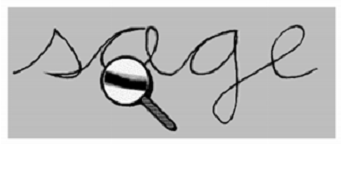
\includegraphics[width=0.5\textwidth]{./figures/offline}
        }
        \subfloat[]{
           \label{fig:online}
           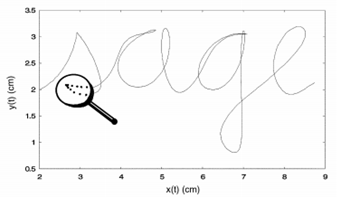
\includegraphics[width=0.5\textwidth]{./figures/online}
        }        
    \caption{(a) Off-line word. The image of the word is converted into gray-level pixels using a scanner. (b) On-line word. The x; y coordinates of the pen-tip are recorded as a function of time with a digitizer \cite{plamondon2000online}.}
   \label{fig:offline_vs_online}
\end{figure}

\iftoggle{edit-mode}{\hspace{0pt}\marginpar{State of the art HWR}}{}
HWR is no longer an esoteric topic on the fringes of information technology, but a mature discipline that has many commercial usages.
On-line systems for handwriting recognition are available in hand-held computers such as PDAs.
Off-line systems are less accurate than on-line systems.
However, they are now good enough that they have a significant economic impact on for specialized domains such as interpreting handwritten postal addresses on envelopes and reading courtesy amounts on bank checks.
The success of on-line systems makes it attractive to consider developing off-line systems that first estimate the trajectory of the writing from off-line data and then use pentip are recorded as a function of time with a digitizer.

\iftoggle{edit-mode}{\hspace{0pt}\marginpar{off-line HWR general recognition scheme}}{}
There are many approaches for off-line handwriting recognition, and it is difficult to draw a common flow or stages that are common on most off-line HWR techniques. One may find it very difficult to draw a general scheme that outlines the flow of off-line handwriting recognition approaches or procedures. However, there are several stages that can be found in many approaches.
\begin{itemize}
\item preprocessing
\item feature extraction
\item classification algorithm
\end{itemize}
The preprocessing stage usually consists of smoothing, writing flow reconstruction, purification, etc... 



\emph{TODO: talk in general about the flow of handwriting recognition and then go into the differences between the off-line and the on-line}\\

\iftoggle{edit-mode}{\hspace{0pt}\marginpar{A general flow for handwriting recognition}}{}
{\color{blue}In a document image, first step is layout analysis and extraction of text lines. Then each text line is segmented into isolated individual character images. In final, these character images are sent to the classifier and the corresponding class labels are obtained. The whole process is straightforward for well printed/well written documents and is shown in Figure \ref{fig:flow_diagram_ocr} \cite{saba2010survey}.}

\begin{figure}
\centering
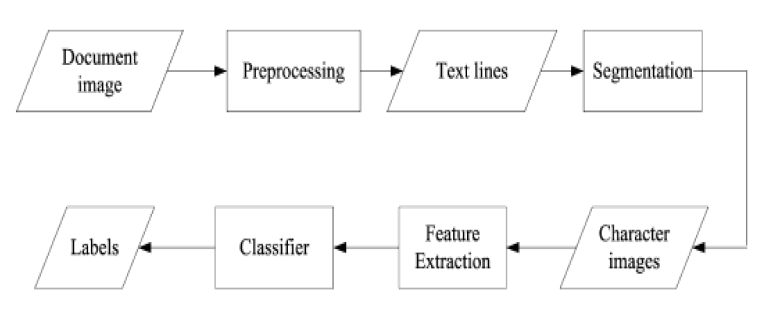
\includegraphics[width=0.7\textwidth]{./figures/flow_diagram_ocr}       
\caption{Generic Handwriting Recognition Process \cite{saba2010survey}}
\label{fig:flow_diagram_ocr}
\end{figure}


\iftoggle{edit-mode}{\hspace{0pt}\marginpar{Common stages of on-line Arabic handwriting recognition system}}{}
As mentioned before, in an on-line handwriting recognition system, the stylos motion is sampled at equal time intervals and pass the information to the recognition algorithm. The samples goes through preprocessing stage that include filtering of noises, re-sampling the stroke information to obtain equidistant stroke, and normalized to a standard size. Additional preprocessing may include slant and slope corrections. Then, depending on the nature of the system, the trajectory may undergoes segmentation into basic units and each unit is labeled, or the word or the WP is classified as a whole. A preprocessing stage usually include using a lexicon/language soecific model to search for the most likely string, see Figure \ref{fig:online_generic_process} \cite{beigi1993overview}. 

\begin{figure}
\centering
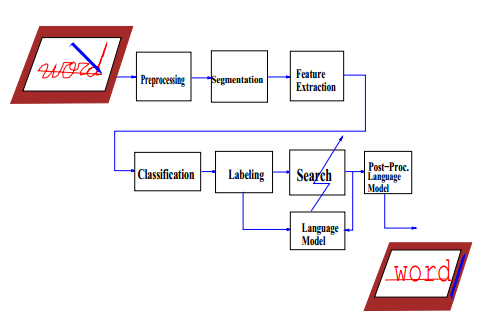
\includegraphics[width=0.7\textwidth]{./figures/online_generic_process}       
\caption{Generic Handwriting Recognition Process \cite{beigi1993overview}}
\label{fig:online_generic_process}
\end{figure}

%%%%%%%%%%%%%%%%%%%%%%%%%%%%%%%%%%%%%%%%%%%%%%
\subsubsection{Closed Vocabulary vs. Open Vocabulary}

\iftoggle{edit-mode}{\hspace{0pt}\marginpar{Importance of the dictionary size}}{}
The vocabulary, from which the words in the test set are taken, has a major impact on how difficult the HWR task is.

\iftoggle{edit-mode}{\hspace{0pt}\marginpar{Closed and open vocabulary definitions}}{}
Closed-vocabulary HWR system is capable of recognizing words from a predetermined limited size dictionary. 
The restricted vocabulary set is usually called a lexicon.
There are no established definitions for the lexicon size, however, the following terms are usually used:
\begin{itemize}
\item small lexicon - tens of words.
\item medium lexicon - hundreds of words.
\item large lexicon - thousands of words.
\item very large lexicon - tens of thousands of words.
\end{itemize}
Open-vocabulary tasks refer to recognition of any words without the constraint of being in a dictionary.

\iftoggle{edit-mode}{\hspace{0pt}\marginpar{Recognition difficulty}}{}
Closed-vocabulary tasks are easier than open-vocabulary ones because only certain subsequences of letters are possible when limited by a dictionary.
The vocabulary size is a common constraint of current recognition systems. 
Most current HWR systems are able to handle small and medium size lexicons.

\iftoggle{edit-mode}{\hspace{0pt}\marginpar{problems imposed by the open vocabulary}}{}
The lexicon is a key-point post-processing stage in many systems, because the linguistic knowledge helps to filter out many possible options that are not included in the lexicon, and consequently raise the recognition rate.
The adhesion to a some limited dictionary, may also limit the computational complexity. 
Although most research efforts have been devoted to closed vocabulary systems, open vocabulary systems has also been proposed.
However, their accuracy is still far below those relying on a small vocabulary \cite{koerich2003large, shu1996line}.
 
%%%%%%%%%%%%%%%%%%%%%%%%%%%%%%%%%%%%%%%%%%%%%%

\subsection{The Holistic versus Analytic approach}

\iftoggle{edit-mode}{\hspace{0pt}\marginpar{problems imposed by the open vocabulary}}{}
While there exist a wide variety of approaches to cursive script recognition, research in this field has established two main approaches
1. the analytic approach \cite{abdulla2008off, sari2002off, Dinges2011, elanwar2012unconstrained} and 2. The holistic approach \cite{biadsy2011segmentation}. 

\iftoggle{edit-mode}{\hspace{0pt}\marginpar{The analytic approach}}{}
The analytic approach involves segmentation of the input curve (that represents a word) into basic units (usually letters) and classification of each part of the text into individual characters, which are recognized and then assembled to identify the written word. 
The advantage of this approach is that it requires to maintain only a small set of trained models - one for each letter shape - to handle large vocabulary. however, the absence of consistent baselines, large variations in writing styles, and seamless connection between letters (connection is done with almost no ligatures)make segmentation into individual letters almost impossible. \cite{saabni2009hierarchical}

\iftoggle{edit-mode}{\hspace{0pt}\marginpar{The holistic approach}}{}
The holistic approach (also called a global approach) considers the global properties of the written text and recognizes the input word shape as a whole. 
{Most popular methods among this group are based on analysis of the number and order of ascenders, descenders, loops and vertical strokes. They often rely on heavy dictionary searching that is costly and prone to be mislead by spelling errors. \cite{brodowska2011oversegmentation}}

While it avoids the error-prone segmentation process the holistic approach, the recognition system needs to be trained over all words in the dictionary and to maintain and train models for each word. 
It may be possible for small vocabulary of words, however, this is not feasible for large vocabularies (20,000 words or more). 
Since each word is constructed from a subset of the character alphabet, it is much more efficient to classify words using the analytic approach \cite{elanwar2012unconstrained}.\\

\iftoggle{edit-mode}{\hspace{0pt}\marginpar{The similarities}}{}
Although HWR processes and approaches may differ, we can safely expect that any OCR algorithm would posses these two essential components:
\begin{itemize}
\item a feature extractor, and
\item a classifier
\end{itemize}
Given an item image, the feature extractor derives the features (descriptors) that the item possesses. The derived features are then used as input to the classifier that determines the (most likely) known item corresponding to the observed features. The classifier is also expected to give a confidence level number that tells how certain the classifier is about the recognized item.


\iftoggle{edit-mode}{\hspace{0pt}\marginpar{Trends in pattern recognitions techniques}}{}
The are some leading pattern recognition techniques, which can be encoutered frequently, when reviewing the field of on-line handwriting recognition.
Techniques such as \emph{hidden Markov models} (HMM) and \emph{neural networks} are encountered frequently.
More details will be provided in Section \ref{}


%%%%%%%%%%%%%%%%%%%%%%%%%%%%%%%%%%%%%%%%%%%%%%%%%%%%%%%
\newpage{}
%%%%%%%%%%%%%%%%%%%%%%%%%%%%%%%%%%%%%%%%%%%%%%%%%%%%%%%

\subsection{Arabic Handwriting Recognition}
\iftoggle{edit-mode}{\hspace{0pt}\marginpar{The Arabic Trend}}{}
After a long period of focus on western and East Asian scripts there is now a general trend to explore other scripts such as Arabic and various Indic scripts. 

%%%%%%%%%%%%%%%%%%%%%%%%%%%%%%%%%%%%%%%%%%%%%%%%%%%%%%%

\subsubsection{Motivation}
\iftoggle{edit-mode}{\hspace{0pt}\marginpar{The Arabic language spread}}{}
The Arabic language is spoken as their first language by nearly 350 million people around the world \cite{zeki2011segmentation}, and written by more than 100 million people, in over 20 different countries, which makes it one of the five most common languages in the world and one of the six United Nations official languages since 1974\cite{burrow2004arabic}. 
Although Arabic is used mainly in the Arab countries, which is about 5.5\% of the world population, almost all Muslims, around 25\% of the world population can read Arabic script as it is the language of the Holy Qur'an \cite{zeki2011segmentation}.


\iftoggle{edit-mode}{\hspace{0pt}\marginpar{The Arabic History}}{}
The Arabic script is one of the descendants of the Aramaic script. 
The earliest known document written using the Arabic script is dating from 512 AD.  
The reason there are some letters in the Arabic script that differ only by dots is the that new letters were created around the 7th century by adding dots to existing Armaic letters \cite{burrow2004arabic}.
The old Arabic was written without dots or diacritics. The dots were first introduced by Yahya bin Ya'mur (died around 746 AD) and Nasr bin Asim (died around 707 AD), students of Abu Al-Aswad Al-Du'ali (died around 688 AD) who introduced the diacritics to prevent the 
Qur'an from being misread by Muslims \cite{zeki2011segmentation}.

\iftoggle{edit-mode}{\hspace{0pt}\marginpar{The Arabic Alphabet usage in other languages}}{}
{Due to the Islamic conquests, the use of Arabic language extended in the 7th and 8th centuries from India to the Atlantic Ocean (Al- Fakhri, 1997). Consequently, more than twenty different languages adopted the Arabic alphabet with some changes, such as Farsi, Urdu, Malay, Housa and Ottoman Turkish \cite{saabni2009efficient,jannoud2007automatic}. }
However, it must be mentioned that some of those languages are currently using Latin characters, but in general, people can still read the Arabic script.

\iftoggle{edit-mode}{\hspace{0pt}\marginpar{Literary vs. daily language}}{}
{The literary language is called Modern Standard Arabic or Literary Arabic which is a Pluricentric language. 
It is currently the only official form of Arabic, used in most written documents as well as in formal spoken occasions, such as lectures and news broadcasts. However, this varies from one country to the other.[wikipedia]}
Other small marks (diacritics) are used to indicate short vowels, often heard and in written when using the standard Arabic are seldom used in day-to-day communication and handwriting. \cite{burrow2004arabic}
Although the spoken Arabic is slightly different from country to country, the written Arabic is standard system used all over the Arab world \cite{saabni2009efficient,jannoud2007automatic}.

\iftoggle{edit-mode}{\hspace{0pt}\marginpar{The growing interest in the Arabic HWR}}{}
{Despite the fact that Arabic alphabets are used in many languages, Arabic Character Recognition (ACR) has not received enough interests from researchers. Little research progress has been achieved as compared to the one done on Latin or Chinese. It has almost only started in 1975 by Nazif (1975), while the earlier research efforts in Latin may be traced back to the middle of the 1940s. However, due to a lack of computing power, no significant work was performed until the 1980s. Recent years have shown a considerable increase in the number of research papers related to ACR. \cite{zeki2011segmentation}}

%%%%%%%%%%%%%%%%%%%%%%%%%%%%%%%%%%%%%%%%%%%%%%%%%%%%%%%

\subsubsection{Characteristic of the Arabic writing system}
Arabic Scripts consists of 28 basic letters, 12 additional special letters, and 8 diacritics. 
Arabic script is written from right to left in a semi-cursive manner in both printed and handwritten. 
Most letters are written in four different letter shapes depending on their position in a word, e.g., the letter \RL{`}  (Ain) appears as \RL{`} (isolated), \RL{`-}(initial),\RL{-`-} (medial) and \RL{-`} (final). Among the basic letters, six are Disconnective - \RL{A} (Alef), \RL{d} (Dal), \RL{_d} (Thal), \RL{r} (Reh), \RL{z} (Zain) and \RL{w} (Waw). 
Disconnective letters do not connect to the following letter and have only two shapes each. 
The presence of this letters interrupts the continuity of the graphic form of a word. 
We denote connected letters in a word, as word-part. 
If the word-part is composed of only one letter, this letter will be in its isolated shape \cite{biadsy2011segmentation}. 

Certain characteristics relating to the obligatory dots and strokes of the Arabic script distinguish it from Roman script, making the recognition of words in Arabic more difficult than in Roman script. First, Most Arabic letters contain dots in addition to the letter body, such as \RL{s} (Sheen) which consists of \RL{s} (Seen) body and three dots above it. In addition to dots, there are stroke that can attach to a letter body creating new letter such as \RL{k}, \RL{.t} and \RL{lA}. These dots and strokes are called delayed strokes since they are usually drawn last in the in handwritten word-part/word. Second, eliminating, adding or moving a dot or stroke could produce a completely different letter and, as a result, produce a word other than the one that was intended (see Table 1). Third, the number of possible variations of delayed strokes is greater than those in Roman scripts, as shown in Figure 2. There are only three such strokes used for English: the cross in the letter t, the slash in x, and the dots in i and j. 

{The Arabic language has some diacritics that are used in the holy book Qur'an and sometimes in teaching material and poetry. These diacritics are small markings used above or below the letters of a word to specify the exact pronunciation of the word. They are not commonly used in the daily, scientific, and business uses, and are not discussed further in this work.\cite{abandah2009analysis}}

\iftoggle{edit-mode}{\hspace{0pt}\marginpar{Word parts count}}{}    
Saabni and El-sana have explored a large collection of Arabic texts and extracted 300,000 different word combinations of 82,000 different word-parts. Ignoring the additional strokes reduced the number of different word-parts to 40,000 \cite{saabni2009efficient}. 

\iftoggle{edit-mode}{\hspace{0pt}\marginpar{Issues with Arabic Handwriting Recognition}}{} 
One difficulty with the Arabic script is the number and position of diacritic marks associated to Arabic characters.
{Recognition and segmentation of Arabic handwritten script is a difficult task because the Arabic handwritten characters are naturally both cursive and unconstrained. The analysis of Arabic script is more complicated in comparison with English script \cite{al2010development}}.

%TODOs:
%\begin{enumerate}
%\item See the section "Overview of Arabic Letters" in \cite{abandah2009analysis}. It talks about letters frequencies and special 
%\item Talk about the WP and give statistics of WP length as described in {abandah2009analysis}
%\item Add a table containing the letters in all positions
%\item See \cite{al2011online}.
%\item See \cite{abandah2009analysis}
%\item TODO:see the in introduction of \cite{abandah2009analysis}
%\item See \cite{lorigo2006offline} - motivation section
%\end{enumerate}

%%%%%%%%%%%%%%%%%%%%%%%%%%%%%%%%%%%%%%%%%%%%%%%%%%%%%%%
\subsection{Arabic script Segmentation}

Character segmentation is the process of splitting the handwritten script into basic units, usually corresponding to single letters or alternatively to different basic units usually named graphems. Graphemes are ... and they could be letters, couples of letters or part of a letter.

\iftoggle{edit-mode}{\hspace{0pt}\marginpar{Importance}}{}
Segmentation is one of the required steps in numerous off-line and on-line cursive handwritten word recognition solutions and has long been a critical area of the OCR process. The problems of segmentation persist today. .
Its importance is derived from the fact that improperly extracted characters are usually difficult to recognize correctly. 
Wrong segmentation will often results in major contribution to the error of the recognition algorithm. 
An integral part of the hand writing recognition process, when the analytic approach is considered, is segmentation. \cite{casey1996survey, brodowska2011oversegmentation}


\iftoggle{edit-mode}{\hspace{0pt}\marginpar{The context dependent of segmentation}}{}
{the segmentation decision is not a local decision, independent of previous and subsequent
decisions. Producing a good match to a library symbol is necessary, but not sufficient, for reliable
recognition. That is, a poor match on a later pattern can cast doubt on the correctness of the current
segmentation/recognition result. Even a series of satisfactory pattern matches can be judged incorrect if
contextual requirements on the system output are not satisfied. For example, the letter sequence "cl" can
often closely resemble a "d", but usually such a choice will not constitute a contextually valid result.}

\iftoggle{edit-mode}{\hspace{0pt}\marginpar{The segmentation - recognition catch-22}}{}
{It is believed, good segmentation is one reason for high accuracy character recognition. However, the task of segmentation, while usually trivial to a human, is a very challenging pattern recognition problem.
The Catch 22 in segmentation is as follows: character is a pattern that
resembles one of the symbols the system is designed to recognize. But to determine such a resemblance
the pattern must be segmented from the document image. Each stage depends on the other, and in complex
cases it is paradoxical to seek a pattern that will match a member of the system's recognition alphabet
of symbols without incorporating detailed knowledge of the structure of those symbols into the process.
\cite{casey1996survey}}

\iftoggle{edit-mode}{\hspace{0pt}\marginpar{Cursive English segmentation - techniques and achievements}}{}
There are many known method of performing cursive letters segmentation. 
The broad range of significant real world applications and the considerable difficulty of the task both contribute to the fact that there are many known methods of performing cursive word recognition - one suited better for some applications and some for the others \cite{brodowska2011oversegmentation}
However, a correct segmentation rate is not easily achievable.

\iftoggle{edit-mode}{\hspace{0pt}\marginpar{The three approaches for segmentation}}{}
In a comprehensive survey done in \cite{casey1996survey}, the authors has pinpointed three elemental strategies for off-line cursive text segmentation in addition to many approaches that are a combinations of these three. They have noted that much of the literature on segmentation reports methods that can be characterized as a blend of these three mentioned methods.

\iftoggle{edit-mode}{\hspace{0pt}\marginpar{Dissection}}{}
The classical approach which is usually named \emph{dissection}. 
This approach attempts to segment the text into character using "character-like" properties. 
Examples of such properties are height, width, separation from neighboring components, disposition along a baseline, etc.
Conventional approaches can segment typical words accurately. 
In this regard, different strategies such as projection profile, bounding box or contour tracing exhibit promising results. 
However, they might lead to incorrect segmentation when deal with touching characters \cite{saba2010survey}.


\iftoggle{edit-mode}{\hspace{0pt}\marginpar{Recognition based segmentation}}{}
The catch 22 described above explains the fact that character segmentation and character classification steps are not totally separate. Degree of connection between them vary from a solution to a solution.
The second approach is recognition-based segmentation, in which the system searches for sub-components in the cursive that match letters in its alphabet. 
In this method, the recognition confidence, heavily affects the overall segmentation accuracy.
The general approach is to split words into segments that should be characters, pass each segment to a classifier and, if the classification results are not satisfactory (e.g. some measure of belief requirements is not met), call segmentation once more with the feedback information about rejecting the previous result. \cite{brodowska2011oversegmentation}

\iftoggle{edit-mode}{\hspace{0pt}\marginpar{The holistic approach}}{}
The holistic methods, in which the system seeks to recognize words as a whole, thus avoiding the segmentation process which was previously discussed in Section \ref{[]}.


\iftoggle{edit-mode}{\hspace{0pt}\marginpar{Over-segmentation}}{}
The most common methods of character segmentation is initial over - segmentation, i.e, finding some set of potential splitting points in the graphical representation of the word and then attempting to eliminate the improper ones
The segmentation task of some cursive and unconstrained nature of some languages such Arabic, anneals the segmentation task. 
The technique requires an over-segmentation stage which partition handwritten words into primitives that may then be processed further to provide the best segmentation.


\iftoggle{edit-mode}{\hspace{0pt}\marginpar{Issues with segmentation}}{}
In languages that are commonly written non-cursively, segmentation techniques may be used in HWR systems.
also may use segmentation techniques since human handwriting 
touching characters are error prone in segmentation stage that contributes to recognition errors.

A through survey on character segmentation is given in \cite{casey1996survey} and \cite{brodowska2011oversegmentation}.  


%References:\\
%--------------\\
%cursive english segmentation [36],[19],[20],[55],[58],[81]
%
%[36] L.D. Harmon, {Automatic Recognition of Print and Script}, Proceedings of the IEEE, vol. 60, no. 10,
%pp. 1165-1177, Oct. 72.
%
%[19] G. Dimauro, S. Impedovo and G. Pirlo, {From Character to Cursive Script Recognition: Future
%Trends in Scientific Research}, Proc. 11th Int. Conf. on Pattern Recognition, vol. II, page 516, Aug.
%1992.
%
%[20] C.E. Dunn and P.S.P. Wang, {Character Segmenting Techniques for Handwritten Text - A Survey},
%Proc. 11th Int. Conf. on Pattern Recognition, vol. II, page 577, August 1992.
%
%[55] E. Lecolinet and O. Baret, {Cursive Word Recognition: Methods and Strategies, Fundamentals in
%Handwriting Recognition}, S. Impedovo (Ed.), NATO ASI Series F: Computer and Systems Sciences,
%vol. 124, Springer Verlag, 1994, pages 235-263.
%
%[81] C.C. Tappert, C.Y. Suen and T. Wakahara, {The State of the Art in On-line Handwriting Recognition},
%IEEE Trans. on Pattern Analysis and Machine Intelligence, vol. 12, no. 8, page 787, Aug.
%1990.

%\bibliographystyle{plainnat}
%\bibliography{references}
%\end{document}
